\section{KV cache 怎么搬}
\label{sec:transfer}

分离把「一次本地写读」变成「一次跨进程或跨机传输」。传输层因此不再
是细节，而是决定分离成败的主变量。

\subsection{三档传输方案}

\begin{table}[t]
\centering
\caption{KV 传输的三档方案。带宽为实测或规格值，比值为相对跨机 RDMA 的
倍数。第三档为推算值，已在文中标注。}
\label{tab:transport}
\small
\begin{tabular}{@{}p{0.9cm}p{1.55cm}p{1.15cm}p{0.72cm}@{}}
\toprule
档位 & 典型承载 & 有效带宽 & 相对 \\
\midrule
同机 & NVLink & 417\,GB/s$^{*}$ & 16.7× \\
跨机 & RDMA / IB & 25\,GB/s$^{*}$ & 1× \\
经存储 & 共享存储 / CXL & $\sim$2.5\,GB/s & $\sim$0.1× \\
\bottomrule
\end{tabular}

\vspace{2pt}
{\footnotesize $^{*}$ 由 e-011 的 250\,MB / 0.6\,ms 与 250\,MB / 10\,ms
反算。第三档是按 RDMA 的 1/10 推算，\textbf{非实测}。}
\end{table}

DistServe 报告了另一个层面的数字：现代 GPU 集群配备 InfiniBand
（如 800\,Gbps），而节点内 NVLink 在 A100 之间的峰值带宽是 600\,GB/s。
按 8 bit/byte 折算，800\,Gbps 约合 100\,GB/s，与 600\,GB/s 相差 6 倍。
DistServe 据此指出：跨节点带宽受限时，分离可以退回到节点内 NVLink，
此时传输开销可以忽略\texttt{[c-transfer]}。

这个「可以退回」很关键——它说明分离的可行性不取决于某一代互联，
而取决于\textbf{是否存在一条带宽足够高的路径}。

\subsection{传输的工程抽象}

NIXL 的做法是把传输差异抽象掉。它的自述是：为推理框架之间的点对点
通信加速，同时通过插件式架构对多种内存（CPU、GPU）与存储（文件、
块设备、对象存储）提供统一抽象\texttt{[c-transfer]}。这样上层的
KV 连接器不必关心底层是 NVLink 还是 RDMA。

工程实现的取舍值得单列。vLLM 的默认 NIXL 连接器是\textbf{拉取式}的：
decode 实例在 prefill 完成后通过 NIXL READ 从 prefill 实例读走 KV 块。
而 push 模式则相反\texttt{[c-transfer]}。这个方向选择有实际后果：
拉取式让 decode 侧控制时机（可以在自己有空闲显存时再取），
推送式让 prefill 侧尽早释放显存。哪个更好取决于哪一侧先成为瓶颈。

\subsection{压缩与精度：直接压低传输量}

既然成本与传输字节数成正比，另一条路是把字节数变小。

SplitZip 走无损压缩路线，报告其压缩比在计入元数据开销后仍比
ZipServ 高 7.1\%，仅比基于 Huffman 的 DFloat11 低 7.0\%\texttt{[c-transfer]}。

SpectrumKV 走逐 token 混合精度路线，其核心结论不是「省了多少带宽」，
而是一个更有意思的判断：\textbf{把全部 token 都降精度，明显优于丢掉一部分
token}。也就是说，对 KV 传输而言，均匀降质比选择性丢弃更划算。

\begin{figure}[t]
  \centering
  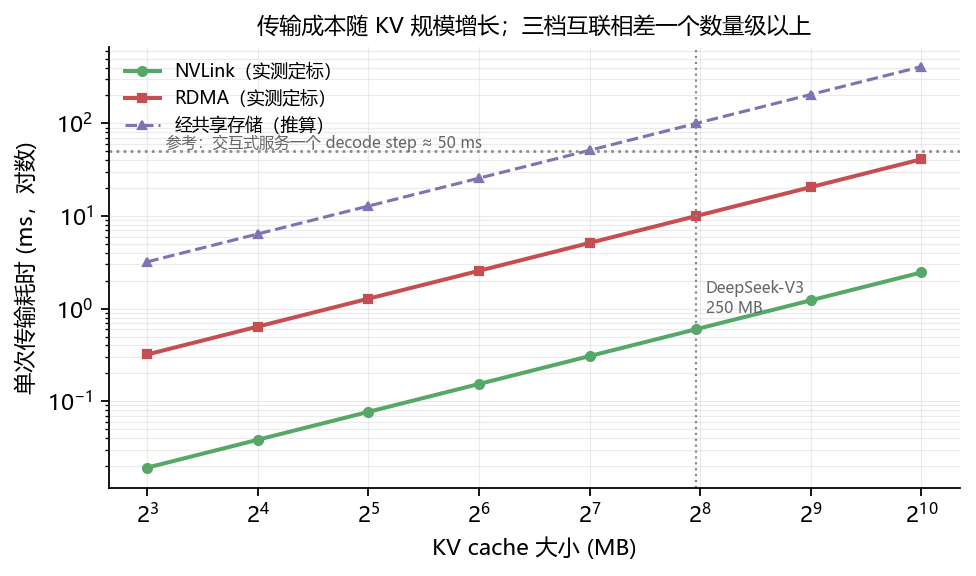
\includegraphics[width=\columnwidth]{figures/fig2_transfer_scaling.png}
  \caption{KV 传输耗时随 KV 规模的增长（对数坐标）。两条实线由
  e-011 的两点实测定标，虚线为按 RDMA 的 1/10 推算的共享存储档，
  \textbf{非实测}。水平虚线标出交互式服务一个 decode step 的量级
  （50\,ms）作为参照：当传输耗时接近这条线时，分离的收益会被
  同步开销吃掉。}
  \label{fig:scaling}
\end{figure}

\subsection{一个必要的提醒}

上面所有带宽数字都是\textbf{峰值或理想条件}下的。实际传输还要付出
同步、建连、内存注册的代价，且这些代价与消息大小不成正比——
小 KV（短上下文、小 batch）时，固定开销占比会急剧上升。

这解释了一个看起来矛盾的现象：短上下文场景下 KV 绝对量小，
按「字节数 ÷ 带宽」算传输应该很快，但实测收益往往不好。
原因是此时固定开销主导，而不是带宽主导\texttt{[c-formula]}。
